\documentclass{anstrans}
%%%%%%%%%%%%%%%%%%%%%%%%%%%%%%%%%%%
\title{Validation of Spent Nuclear Fuel Output by Cyclus, a Fuel Cycle Simulator Code}
\author{Gwendolyn J. Chee, Gyutae Park, and Kathryn D. Huff}

\institute{
Dept. of Nuclear, Plasma and Radiological Engineering, University of Illinois at Urbana-Champaign \\
gchee2@illinois.edu
}

%%%% packages and definitions (optional)
\usepackage{graphicx} % allows inclusion of graphics
\usepackage{booktabs} % nice rules (thick lines) for tables
\usepackage{microtype} % improves typography for PDF
\usepackage{xspace}
\usepackage{tabularx}
\usepackage{subcaption}
\usepackage{enumitem}
\usepackage{placeins}
\usepackage[acronym,toc]{glossaries}
%\newacronym{<++>}{<++>}{<++>}
\newacronym[longplural={metric tons of heavy metal}]{MTHM}{MTHM}{metric ton of heavy metal}
\newacronym{ABM}{ABM}{agent-based modeling}
\newacronym{ACDIS}{ACDIS}{Program in Arms Control \& Domestic and International Security}
\newacronym{AHTR}{AHTR}{Advanced High Temperature Reactor}
\newacronym{ANDRA}{ANDRA}{Agence Nationale pour la gestion des D\'echets RAdioactifs, the French National Agency for Radioactive Waste Management}
\newacronym{ANL}{ANL}{Argonne National Laboratory}
\newacronym{API}{API}{application programming interface}
\newacronym{ARE}{ARE}{Aircraft Reactor Experiment}
\newacronym{ARFC}{ARFC}{Advanced Reactors and Fuel Cycles}
\newacronym{ASME}{ASME}{American Society of Mechanical Engineers}
\newacronym{ATWS}{ATWS}{Anticipated Transient Without Scram}
\newacronym{BDBE}{BDBE}{Beyond Design Basis Event}
\newacronym{BIDS}{BIDS}{Berkeley Institute for Data Science}
\newacronym{CAFCA}{CAFCA}{ Code for Advanced Fuel Cycles Assessment }
\newacronym{CDTN}{CDTN}{Centro de Desenvolvimento da Tecnologia Nuclear}
\newacronym{CEA}{CEA}{Commissariat \`a l'\'Energie Atomique et aux \'Energies Alternatives}
\newacronym{CI}{CI}{continuous integration}
\newacronym{CNEN}{CNEN}{Comiss\~{a}o Nacional de Energia Nuclear}
\newacronym{CNERG}{CNERG}{Computational Nuclear Engineering Research Group}
\newacronym{COSI}{COSI}{Commelini-Sicard}
\newacronym{COTS}{COTS}{commercial, off-the-shelf}
\newacronym{CSNF}{CSNF}{commercial spent nuclear fuel}
\newacronym{CTAH}{CTAHs}{Coiled Tube Air Heaters}
\newacronym{CUBIT}{CUBIT}{CUBIT Geometry and Mesh Generation Toolkit}
\newacronym{CURIE}{CURIE}{Centralized Used Fuel Resource for Information Exchange}
\newacronym{DAG}{DAG}{directed acyclic graph}
\newacronym{DANESS}{DANESS}{Dynamic Analysis of Nuclear Energy System Strategies}
\newacronym{DBE}{DBE}{Design Basis Event}
\newacronym{DESAE}{DESAE}{Dynamic Analysis of Nuclear Energy Systems Strategies}
\newacronym{DHS}{DHS}{Department of Homeland Security}
\newacronym{DOE}{DOE}{Department of Energy}
\newacronym{DRACS}{DRACS}{Direct Reactor Auxiliary Cooling System}
\newacronym{DRE}{DRE}{dynamic resource exchange}
\newacronym{DSNF}{DSNF}{DOE spent nuclear fuel}
\newacronym{DYMOND}{DYMOND}{Dynamic Model of Nuclear Development }
\newacronym{EBS}{EBS}{Engineered Barrier System}
\newacronym{EDZ}{EDZ}{Excavation Disturbed Zone}
\newacronym{EIA}{EIA}{U.S. Energy Information Administration}
\newacronym{EPA}{EPA}{Environmental Protection Agency}
\newacronym{EP}{EP}{Engineering Physics}
\newacronym{FCO}{FCO}{Fuel Cycle Options}
\newacronym{FCT}{FCT}{Fuel Cycle Technology}
\newacronym{FEHM}{FEHM}{Finite Element Heat and Mass Transfer}
\newacronym{FEPs}{FEPs}{Features, Events, and Processes}
\newacronym{FHR}{FHR}{Fluoride-Salt-Cooled High-Temperature Reactor}
\newacronym{FLiBe}{FLiBe}{Fluoride-Lithium-Beryllium}
\newacronym{GDSE}{GDSE}{Generic Disposal System Environment}
\newacronym{GDSM}{GDSM}{Generic Disposal System Model}
\newacronym{GENIUSv1}{GENIUSv1}{Global Evaluation of Nuclear Infrastructure Utilization Scenarios, Version 1}
\newacronym{GENIUSv2}{GENIUSv2}{Global Evaluation of Nuclear Infrastructure Utilization Scenarios, Version 2}
\newacronym{GENIUS}{GENIUS}{Global Evaluation of Nuclear Infrastructure Utilization Scenarios}
\newacronym{GPAM}{GPAM}{Generic Performance Assessment Model}
\newacronym{GRSAC}{GRSAC}{Graphite Reactor Severe Accident Code}
\newacronym{GUI}{GUI}{graphical user interface}
\newacronym{HLW}{HLW}{high level waste}
\newacronym{HPC}{HPC}{high-performance computing}
\newacronym{HTC}{HTC}{high-throughput computing}
\newacronym{HTGR}{HTGR}{High Temperature Gas-Cooled Reactor}
\newacronym{IAEA}{IAEA}{International Atomic Energy Agency}
\newacronym{IEMA}{IEMA}{Illinois Emergency Mangament Agency}
\newacronym{INL}{INL}{Idaho National Laboratory}
\newacronym{IPRR1}{IRP-R1}{Instituto de Pesquisas Radioativas Reator 1}
\newacronym{IRP}{IRP}{Integrated Research Project}
\newacronym{ISFSI}{ISFSI}{Independent Spent Fuel Storage Installation}
\newacronym{ISRG}{ISRG}{Independent Student Research Group}
\newacronym{JFNK}{JFNK}{Jacobian-Free Newton Krylov}
\newacronym{LANL}{LANL}{Los Alamos National Laboratory}
\newacronym{LBNL}{LBNL}{Lawrence Berkeley National Laboratory}
\newacronym{LCOE}{LCOE}{levelized cost of electricity}
\newacronym{LDRD}{LDRD}{laboratory directed research and development}
\newacronym{LFR}{LFR}{Lead-Cooled Fast Reactor}
\newacronym{LLNL}{LLNL}{Lawrence Livermore National Laboratory}
\newacronym{LMFBR}{LMFBR}{Liquid Metal Fast Breeder Reactor}
\newacronym{LOFC}{LOFC}{Loss of Forced Cooling}
\newacronym{LOHS}{LOHS}{Loss of Heat Sink}
\newacronym{LOLA}{LOLA}{Loss of Large Area}
\newacronym{LP}{LP}{linear program}
\newacronym{MA}{MA}{minor actinide}
\newacronym{MCNP}{MCNP}{Monte Carlo N-Particle code}
\newacronym{MILP}{MILP}{mixed-integer linear program}
\newacronym{MIT}{MIT}{the Massachusetts Institute of Technology}
\newacronym{MOAB}{MOAB}{Mesh-Oriented datABase}
\newacronym{MOOSE}{MOOSE}{Multiphysics Object-Oriented Simulation Environment}
\newacronym{MOX}{MOX}{mixed oxide}
\newacronym{MSBR}{MSBR}{Molten Salt Breeder Reactor}
\newacronym{MSRE}{MSRE}{Molten Salt Reactor Experiment}
\newacronym{MSR}{MSR}{Molten Salt Reactor}
\newacronym{NAGRA}{NAGRA}{National Cooperative for the Disposal of Radioactive Waste}
\newacronym{NEAMS}{NEAMS}{Nuclear Engineering Advanced Modeling and Simulation}
\newacronym{NEUP}{NEUP}{Nuclear Energy University Programs}
\newacronym{NFCSim}{NFCSim}{Nuclear Fuel Cycle Simulator}
\newacronym{NGNP}{NGNP}{Next Generation Nuclear Plant}
\newacronym{NMWPC}{NMWPC}{Nuclear MW Per Capita}
\newacronym{NNSA}{NNSA}{National Nuclear Security Administration}
\newacronym{NPRE}{NPRE}{Department of Nuclear, Plasma, and Radiological Engineering}
\newacronym{NQA1}{NQA-1}{Nuclear Quality Assurance - 1}
\newacronym{NRC}{NRC}{Nuclear Regulatory Commission}
\newacronym{NSF}{NSF}{National Science Foundation}
\newacronym{NSSC}{NSSC}{Nuclear Science and Security Consortium}
\newacronym{NUWASTE}{NUWASTE}{Nuclear Waste Assessment System for Technical Evaluation}
\newacronym{NWF}{NWF}{Nuclear Waste Fund}
\newacronym{NWTRB}{NWTRB}{Nuclear Waste Technical Review Board}
\newacronym{OCRWM}{OCRWM}{Office of Civilian Radioactive Waste Management}
\newacronym{ORION}{ORION}{ORION}
\newacronym{ORNL}{ORNL}{Oak Ridge National Laboratory}
\newacronym{PARCS}{PARCS}{Purdue Advanced Reactor Core Simulator}
\newacronym{PBAHTR}{PB-AHTR}{Pebble Bed Advanced High Temperature Reactor}
\newacronym{PBFHR}{PB-FHR}{Pebble-Bed Fluoride-Salt-Cooled High-Temperature Reactor}
\newacronym{PEI}{PEI}{Peak Environmental Impact}
\newacronym{PH}{PRONGHORN}{PRONGHORN}
\newacronym{PRKE}{PRKE}{Point Reactor Kinetics Equations}
\newacronym{PSPG}{PSPG}{Pressure-Stabilizing/Petrov-Galerkin}
\newacronym{PWAR}{PWAR}{Pratt and Whitney Aircraft Reactor}
\newacronym{PWR}{PWR}{Pressurized Water Reactor}
\newacronym{PyNE}{PyNE}{Python toolkit for Nuclear Engineering}
\newacronym{PyRK}{PyRK}{Python for Reactor Kinetics}
\newacronym{QA}{QA}{quality assurance}
\newacronym{RDD}{RD\&D}{Research Development and Demonstration}
\newacronym{RD}{R\&D}{Research and Development}
\newacronym{RELAP}{RELAP}{Reactor Excursion and Leak Analysis Program}
\newacronym{RIA}{RIA}{Reactivity Insertion Accident}
\newacronym{RIF}{RIF}{Region-Institution-Facility}
\newacronym{SFR}{SFR}{Sodium-Cooled Fast Reactor}
\newacronym{SINDAG}{SINDA{\textbackslash}G}{Systems Improved Numerical Differencing Analyzer $\backslash$ Gaski}
\newacronym{SKB}{SKB}{Svensk K\"{a}rnbr\"{a}nslehantering AB}
\newacronym{SNF}{SNF}{spent nuclear fuel}
\newacronym{SNL}{SNL}{Sandia National Laboratory}
\newacronym{STC}{STC}{specific temperature change}
\newacronym{SUPG}{SUPG}{Streamline-Upwind/Petrov-Galerkin}
\newacronym{SWF}{SWF}{Separations and Waste Forms}
\newacronym{SWU}{SWU}{Separative Work Unit}
\newacronym{TRIGA}{TRIGA}{Training Research Isotope General Atomic}
\newacronym{TRISO}{TRISO}{Tristructural Isotropic}
\newacronym{TSM}{TSM}{Total System Model}
\newacronym{TSPA}{TSPA}{Total System Performance Assessment for the Yucca Mountain License Application}
\newacronym{ThOX}{ThOX}{thorium oxide}
\newacronym{UFD}{UFD}{Used Fuel Disposition}
\newacronym{UML}{UML}{Unified Modeling Language}
\newacronym{UOX}{UOX}{uranium oxide}
\newacronym{UQ}{UQ}{uncertainty quantification}
\newacronym{US}{US}{United States}
\newacronym{UW}{UW}{University of Wisconsin}
\newacronym{VISION}{VISION}{the Verifiable Fuel Cycle Simulation Model}
\newacronym{VV}{V\&V}{verification and validation}
\newacronym{WIPP}{WIPP}{Waste Isolation Pilot Plant}
\newacronym{YMR}{YMR}{Yucca Mountain Repository Site}

\makeglossaries
\newcommand{\SN}{S$_N$}
\renewcommand{\vec}[1]{\bm{#1}} %vector is bold italic
\newcommand{\vd}{\bm{\cdot}} % slightly bold vector dot
\newcommand{\grad}{\vec{\nabla}} % gradient
\newcommand{\ud}{\mathop{}\!\mathrm{d}} % upright derivative symbol
\newcommand{\Cyclus}{\textsc{Cyclus}\xspace}%
\newcommand{\Cycamore}{\textsc{Cycamore}\xspace}%
\newcolumntype{c}{>{\hsize=.56\hsize}X}
\newcolumntype{b}{>{\hsize=.7\hsize}X}
\newcolumntype{s}{>{\hsize=.74\hsize}X}
\newcolumntype{f}{>{\hsize=.1\hsize}X}
\newcolumntype{a}{>{\hsize=.45\hsize}X}
\usepackage{titlesec}
\titleformat*{\subsection}{\normalfont}

\begin{document}
%%%%%%%%%%%%%%%%%%%%%%%%%%%%%%%%%%%%%%%%%%%%%%%%%%%%%%%%%%%%%%%%%%%%%%%%%%%%%%%%
\section{Introduction}
\Cyclus \cite{carlsen_cyclus_2014}, a nuclear fuel cycle simulator, was used to simulate the
United States' nuclear fuel cycle from 1967 through 2013. The spent nuclear 
\gls{SNF} inventory from the \Cyclus simulation was compared to the \gls{SNF} 
inventory from the \gls{DOE} sponsored \gls{UNFSTANDARDS} \gls{UDB} 
\cite{peterson_unf-st&dards_2017}. The \gls{UDB} provides comprehensive and 
consistent technical data on reactor sites and \gls{SNF} from the beginning of 
nuclear reactor operation in the \gls{US} until 2013. This comparison 
between \Cyclus and \gls{UDB} establishes a realistic validation of \Cyclus' 
capability to produce total spent fuel mass and accurate isotopic compositions 
that closely match reality.

%%% 
\section{Background}
\Cyclus is an agent-based nuclear fuel cycle simulation framework 
\cite{huff_fundamental_2016}, which means that each entity (i.e. Region, 
Institution, or Facility) in the fuel cycle is modeled as an agent. 
\Cycamore \cite{carlsen_cycamore_2014} provides agents to represent process 
physics of various components of the nuclear fuel cycle (e.g. mine, fuel 
enrichment facility, reactor) \cite{huff_extensions_2014}. The nuclear fuel 
assemblies tracked within the simulation are recipe-based. Recipes specify mass 
fractions for each isotope for fresh and spent fuel. They are calculated ahead 
of time using neutronics depletion analysis tools such as ORIGEN 
\cite{bell_origen_1973}, then entered directly into the fuel cycle simulation 
\cite{peterson_additional_2017}. 

%%%%%%%%%%%%%%%%%%%%%%%%%%%%%%%%%%%%%%%%%%%%%%%%%%%%%%%%%%%%%%%%%%%%%%%%%%%%%%%%
\section{Motivation}
The \gls{US} is currently considering various and geologic disposal 
options \cite{DOE_strategy_2013}. Decisions such as waste package spacing, 
waste repository size, and geometry will be influenced by key criteria such as 
thermal load of waste packages and the thermal capacity of the selected 
geologic host media. Waste package thermal evolution depends on the decay heat 
contribution from each isotope in the spent fuel. Therefore, to correctly 
simulate loading of a waste repository based on thermal constraints in \Cyclus, 
the simulation must first give isotopic compositions and spent fuel masses that 
closely replicate reality. 

%%%%%%%%%%%%%%%%%%%%%%%%%%%%%%%%%%%%%%%%%%%%%%%%%%%%%%%%%%%%%%%%%%%%%%%%%%%%%%%%
\section{Methodology}
A \Cyclus simulation of the \gls{US} nuclear fuel cycle was created using 
published data of the 112 commerical nuclear reactors that have operated since 
1967 in the \gls{US}. The reactor deployment data was obtained from \gls{PRIS} 
reactor database \cite{IAEA_pris_2017}.  Relevant data includes country, 
reactor unit, reactor type, net capacity (MWe), first grid date, and shutdown 
date. \gls{US}' reactor data was extracted and used to populate the \Cyclus 
simulation. The recipes used in the \Cyclus simulations are taken from a 
reference depletion calculation done using ORIGEN \cite{bell_origen_1973} for 
burnups of 51 and 33 GWD/MTU. They were also used in 
\cite{wilson_adoption_2009, bae_synergistic_2017}. 

Jinja2 \cite{ronacher_welcome_2018}, a Python templating language, was then 
used in Python to render the data into an input file that is accepted by 
\Cyclus. The output file produced by \Cyclus was also analyzed using Python. 

The assumptions made for this \Cyclus simulation include: 

\begin{enumerate}[topsep=0pt,itemsep=-1ex,partopsep=1ex,parsep=1ex]
	\item Cycle time is assumed to be 18 months. 
	\item Refueling time is assumed to be 1 month. 
	\item There is isotopic decay. 
\end{enumerate}

The \gls{UDB} database contains commercial \gls{SNF} information from 1967 through 2013. 
Data such as initial enrichment, burnup, mass of spent fuel and discharged 
dates were collected from multiple sources \cite{peterson_additional_2017}. 
Meanwhile, data such as isotopic compositions, heat and activity were determined 
by performing irradiation and decay calculations on every fuel assembly based 
on the collected data. 

The \gls{UDB} dataset used for this work included discharged fuel assembly data per 
reactor, specific isotopic concentrations and decay heat for each assembly 
along with its discharge date \cite{peterson_unf-st&dards_2017}. The \gls{UDB} 
dataset was imported into Python, processed and compared with \Cyclus 
simulation output. All scripts and data used are available in 
\cite{chee_arfc/transition-scenarios_2018}. 
%%%%%%%%%%%%%%%%%%%%%%%%%%%%%%%%%%%%%%%%%%%%%%%%%%%%%%%%%%%%%%%%%%%%%%%%%%%%%%%%
\section{Results and Analysis}
The primary outcome of this validation is to provide comparisons between 
\Cyclus data and \gls{UDB} data for spent fuel mass and isotopic contributions to the 
spent fuel mass. 

\subsection{\textit{Cumulative Total Spent Fuel Mass Comparison}}
Figure \ref{fig:total_original} shows the cumulative spent fuel mass for both 
\Cyclus and \gls{UDB} data from 1967 to 2013. The spent fuel mass estimated by 
\Cyclus is larger than the \gls{UDB} calculation before the year 2000. After 2000,
the \gls{UDB} calculation reports a larger spent fuel mass. The discrepancies can be 
attributed to rigidity of \Cyclus simulation input with respect to cycle and 
refueling duration. In \Cyclus, the user specifies refueling and cycle times for each 
reactor as constant integer months.  In reality, the cycle and refueling durations 
vary throughout each reactor's lifetime and are not exact integer multiples of 
one month. 

\begin{figure}[t] % replace 't' with 'b' to force it to be on the bottom
	\centering
	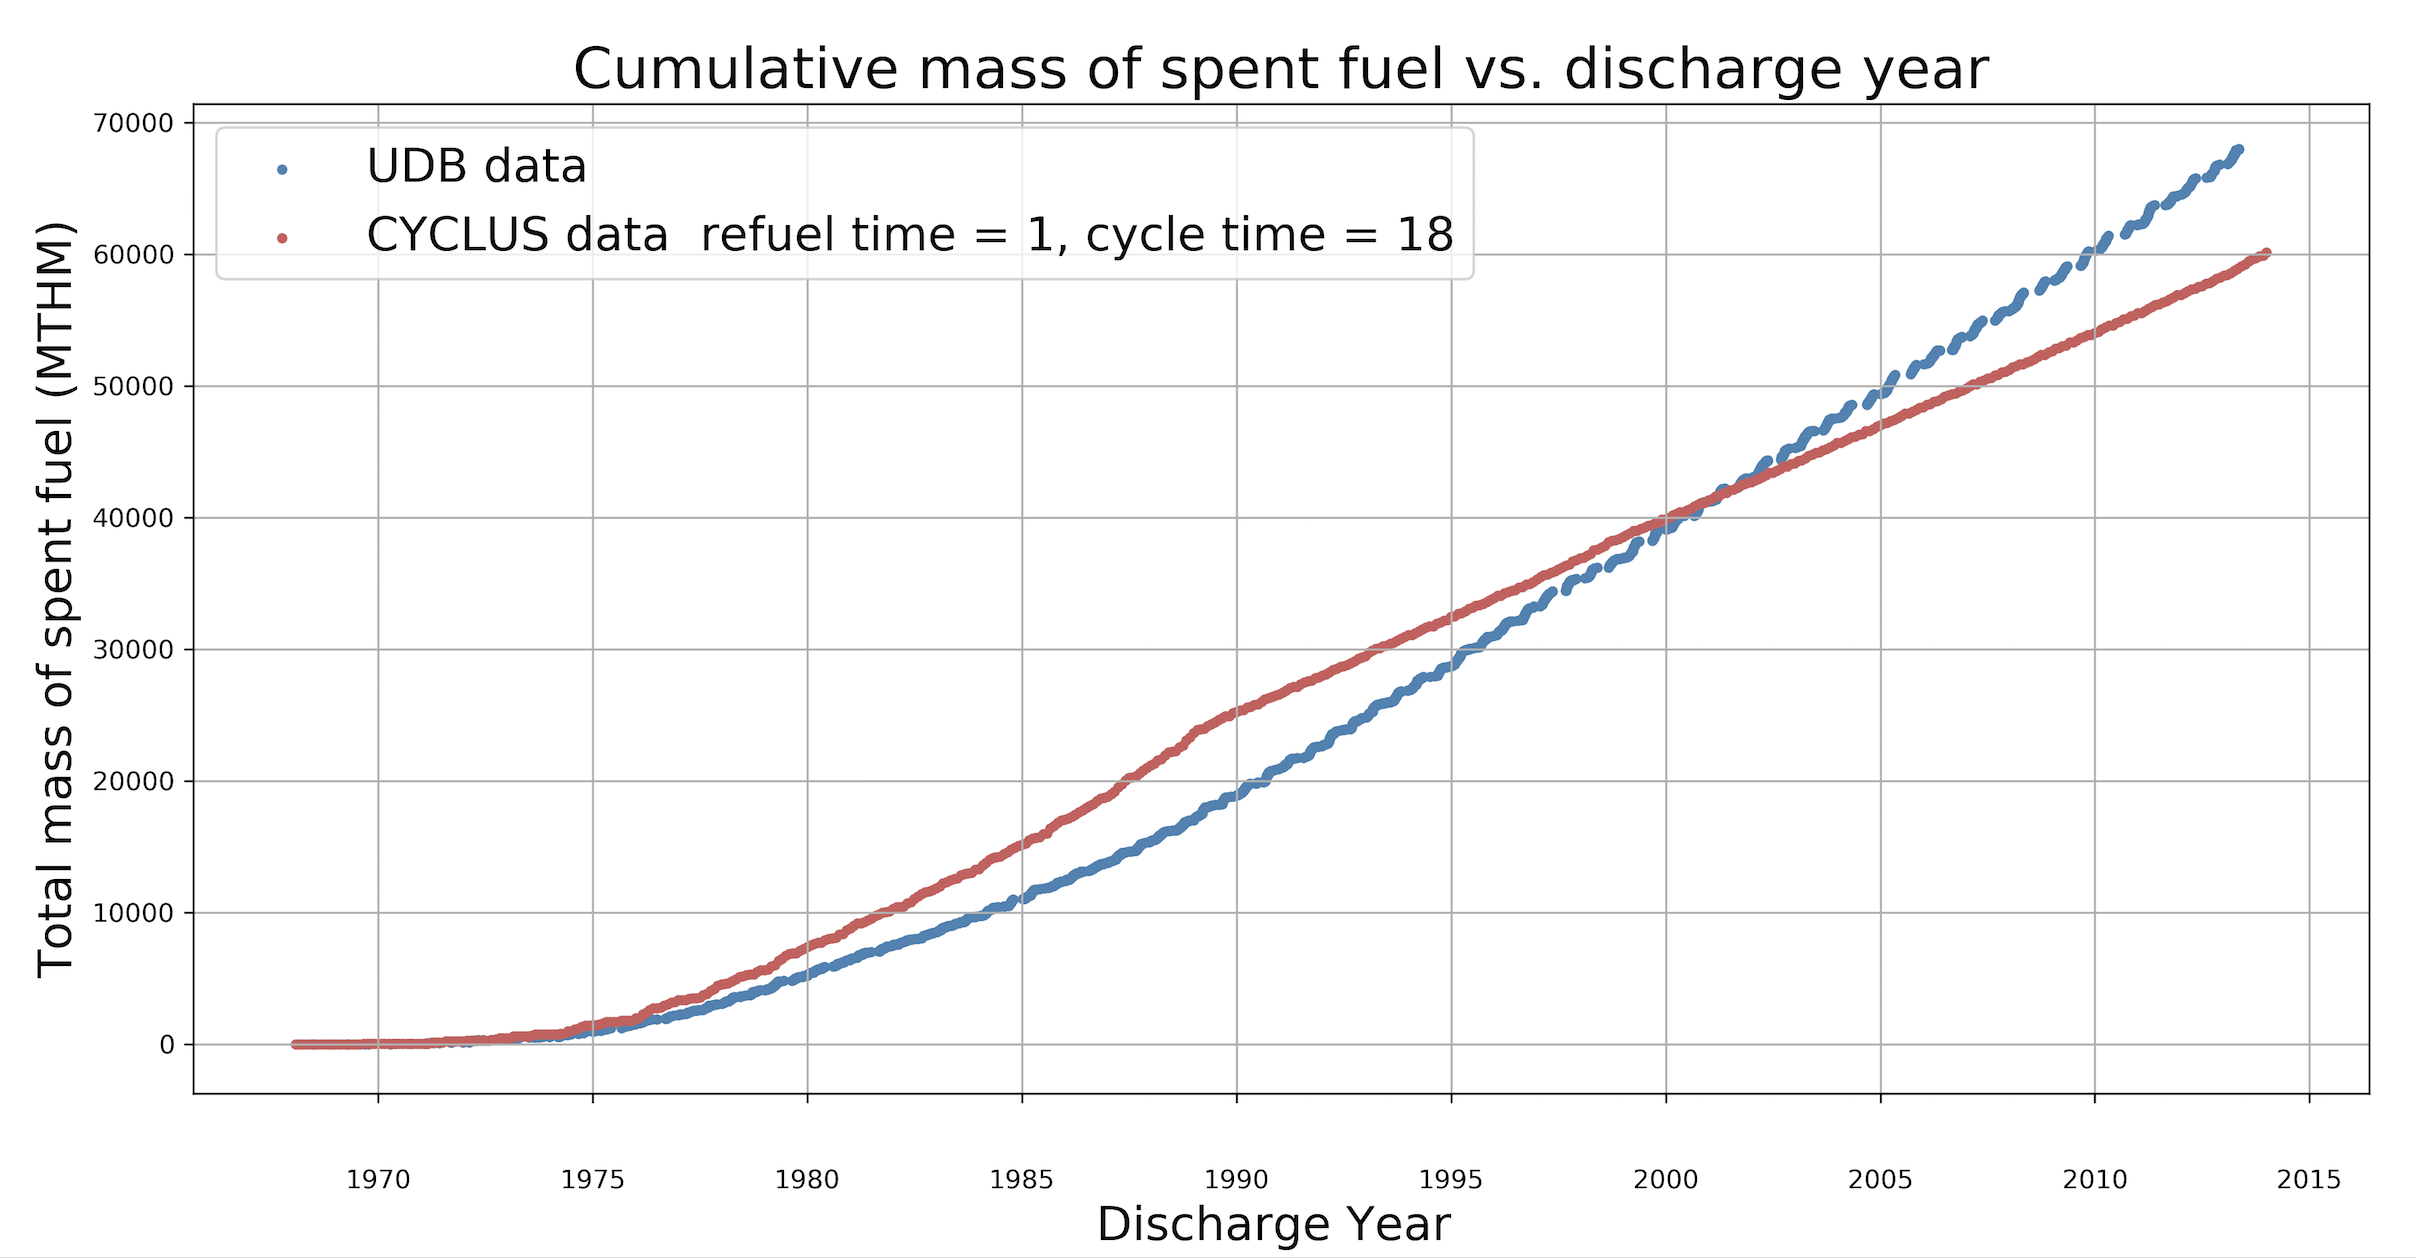
\includegraphics[width=0.48\textwidth]{figures/total_cumulative_mass_spent_fuel_original}
	\caption{The total cumulative spent fuel mass against discharge time for \Cyclus and \gls{UDB} data from 1967 through 2013.}
	\label{fig:total_original}
\end{figure}

The \gls{NEI} reported significant 
variance in the refueling period for \gls{US} reactors. While average 
refuelling time in 1990 was 104 days, it decreased to an average 
refuelling time of 35 days in 2017 \cite{iaea_current_nodate}.

Figure \ref{fig:total_refueltime} includes plots of total spent fuel mass from 
\Cyclus simulations where refueling duration is increased. A longer refueling duration brings 
the total spent fuel mass from \Cyclus simulations closer to the \gls{UDB} data 
before 2000. 

\begin{figure}[t] 
	\centering
	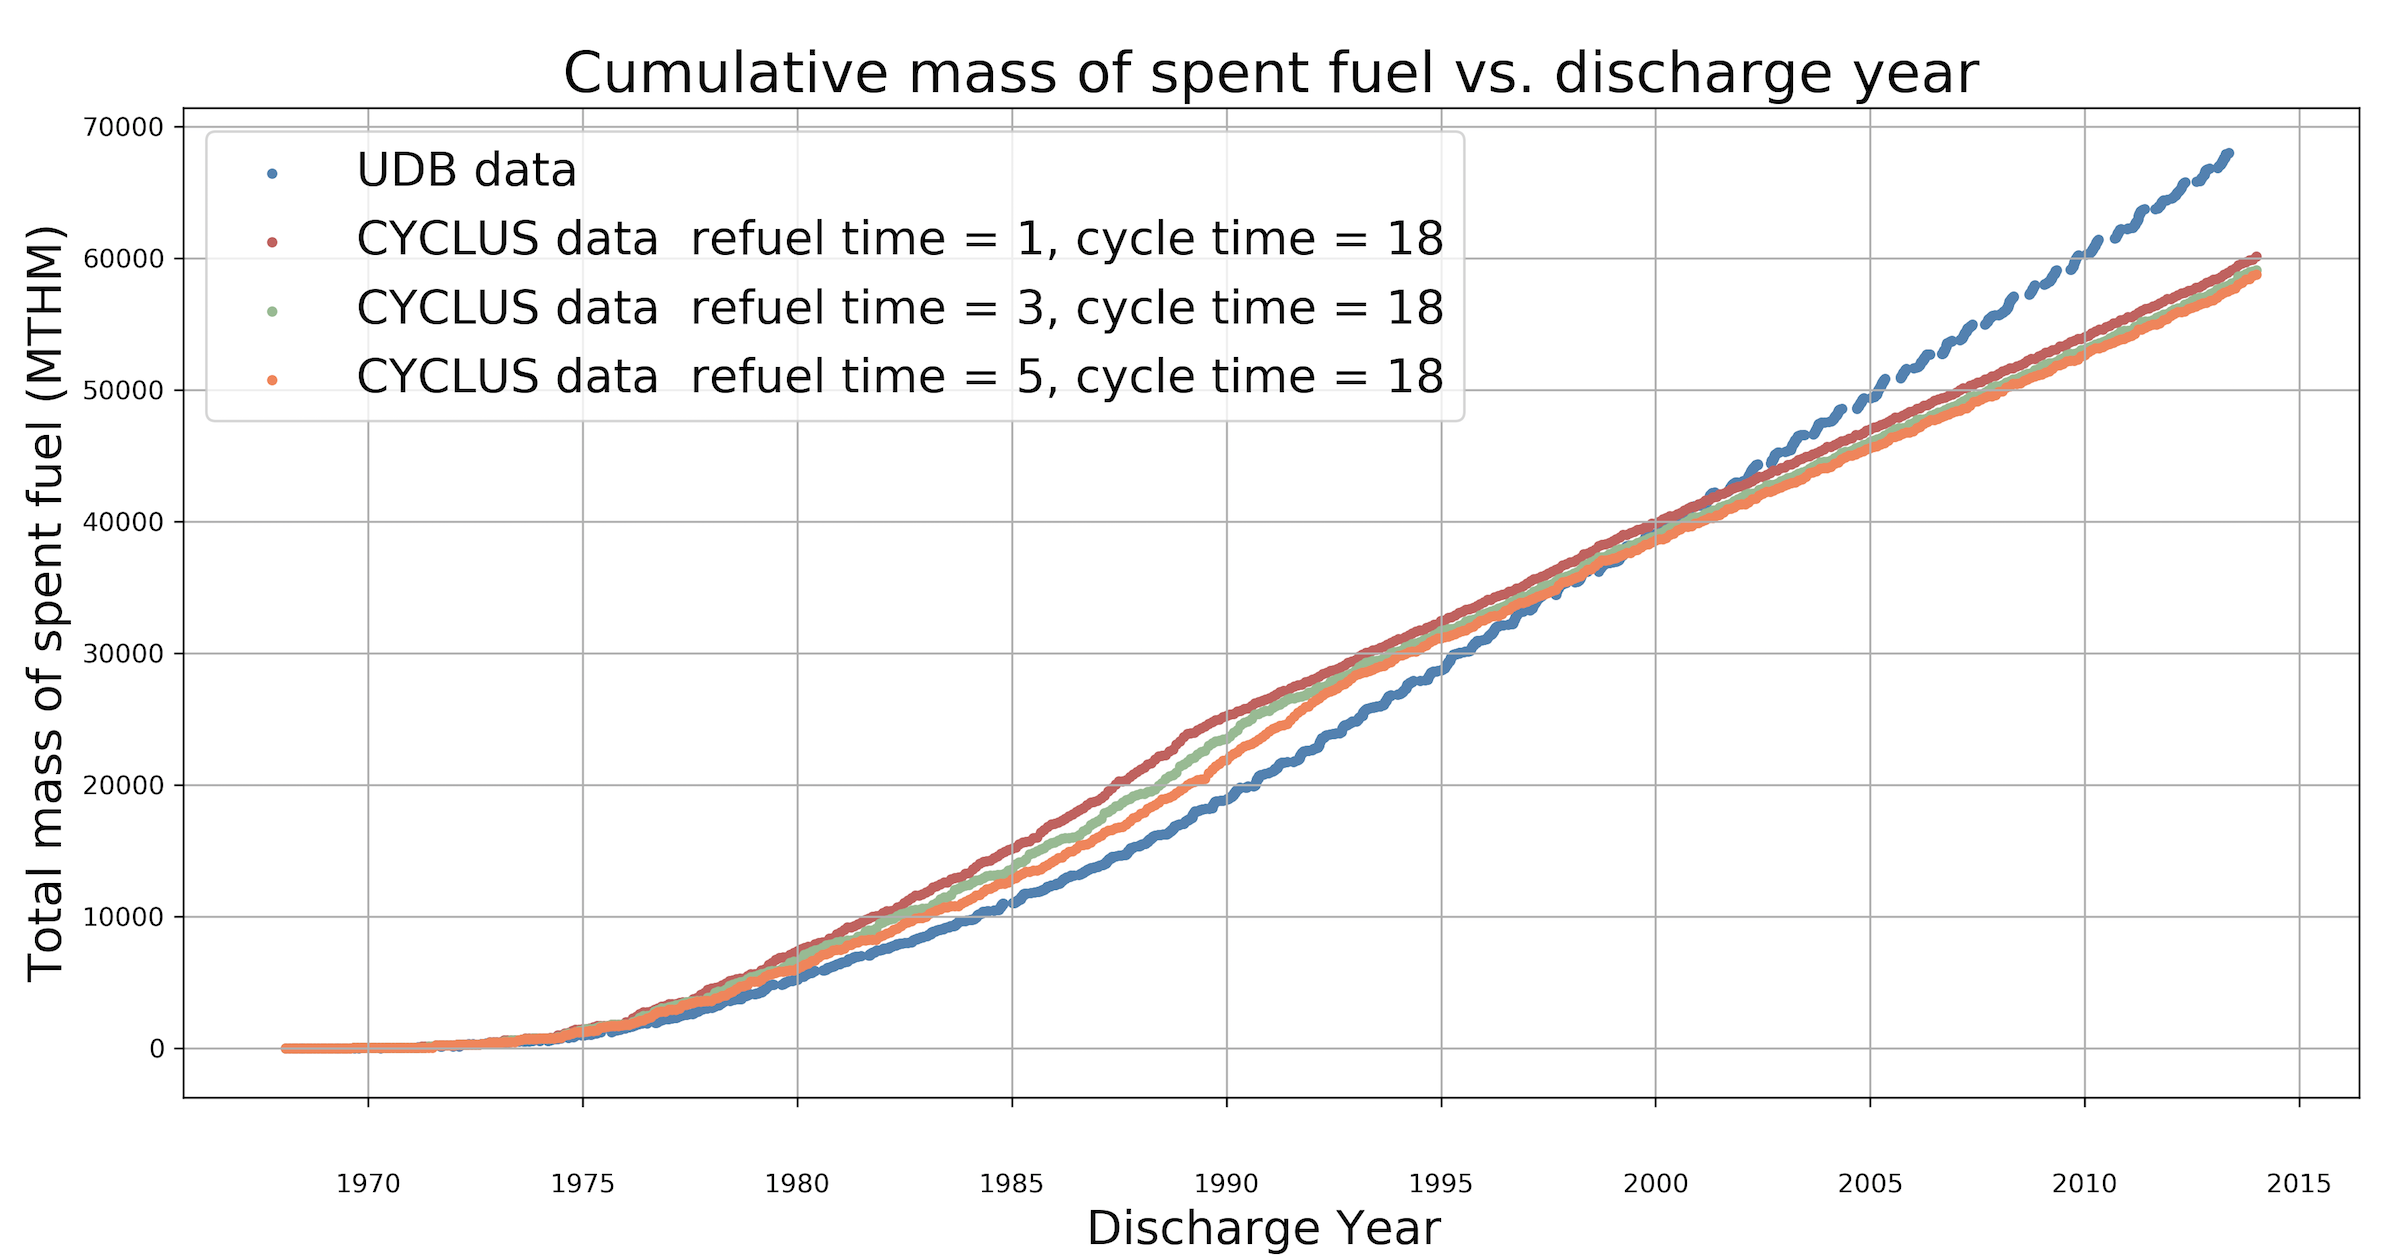
\includegraphics[width=0.48\textwidth]{figures/total_cumulative_mass_spent_fuel_refueltime}
	\caption{The total cumulative spent fuel mass against discharge time for \Cyclus and \gls{UDB} data from 1967 through 2013 for various refueling durations.}
	\label{fig:total_refueltime}
\end{figure} 

\begin{figure}[b] % replace 't' with 'b' to force it to be on the bottom
	\centering
	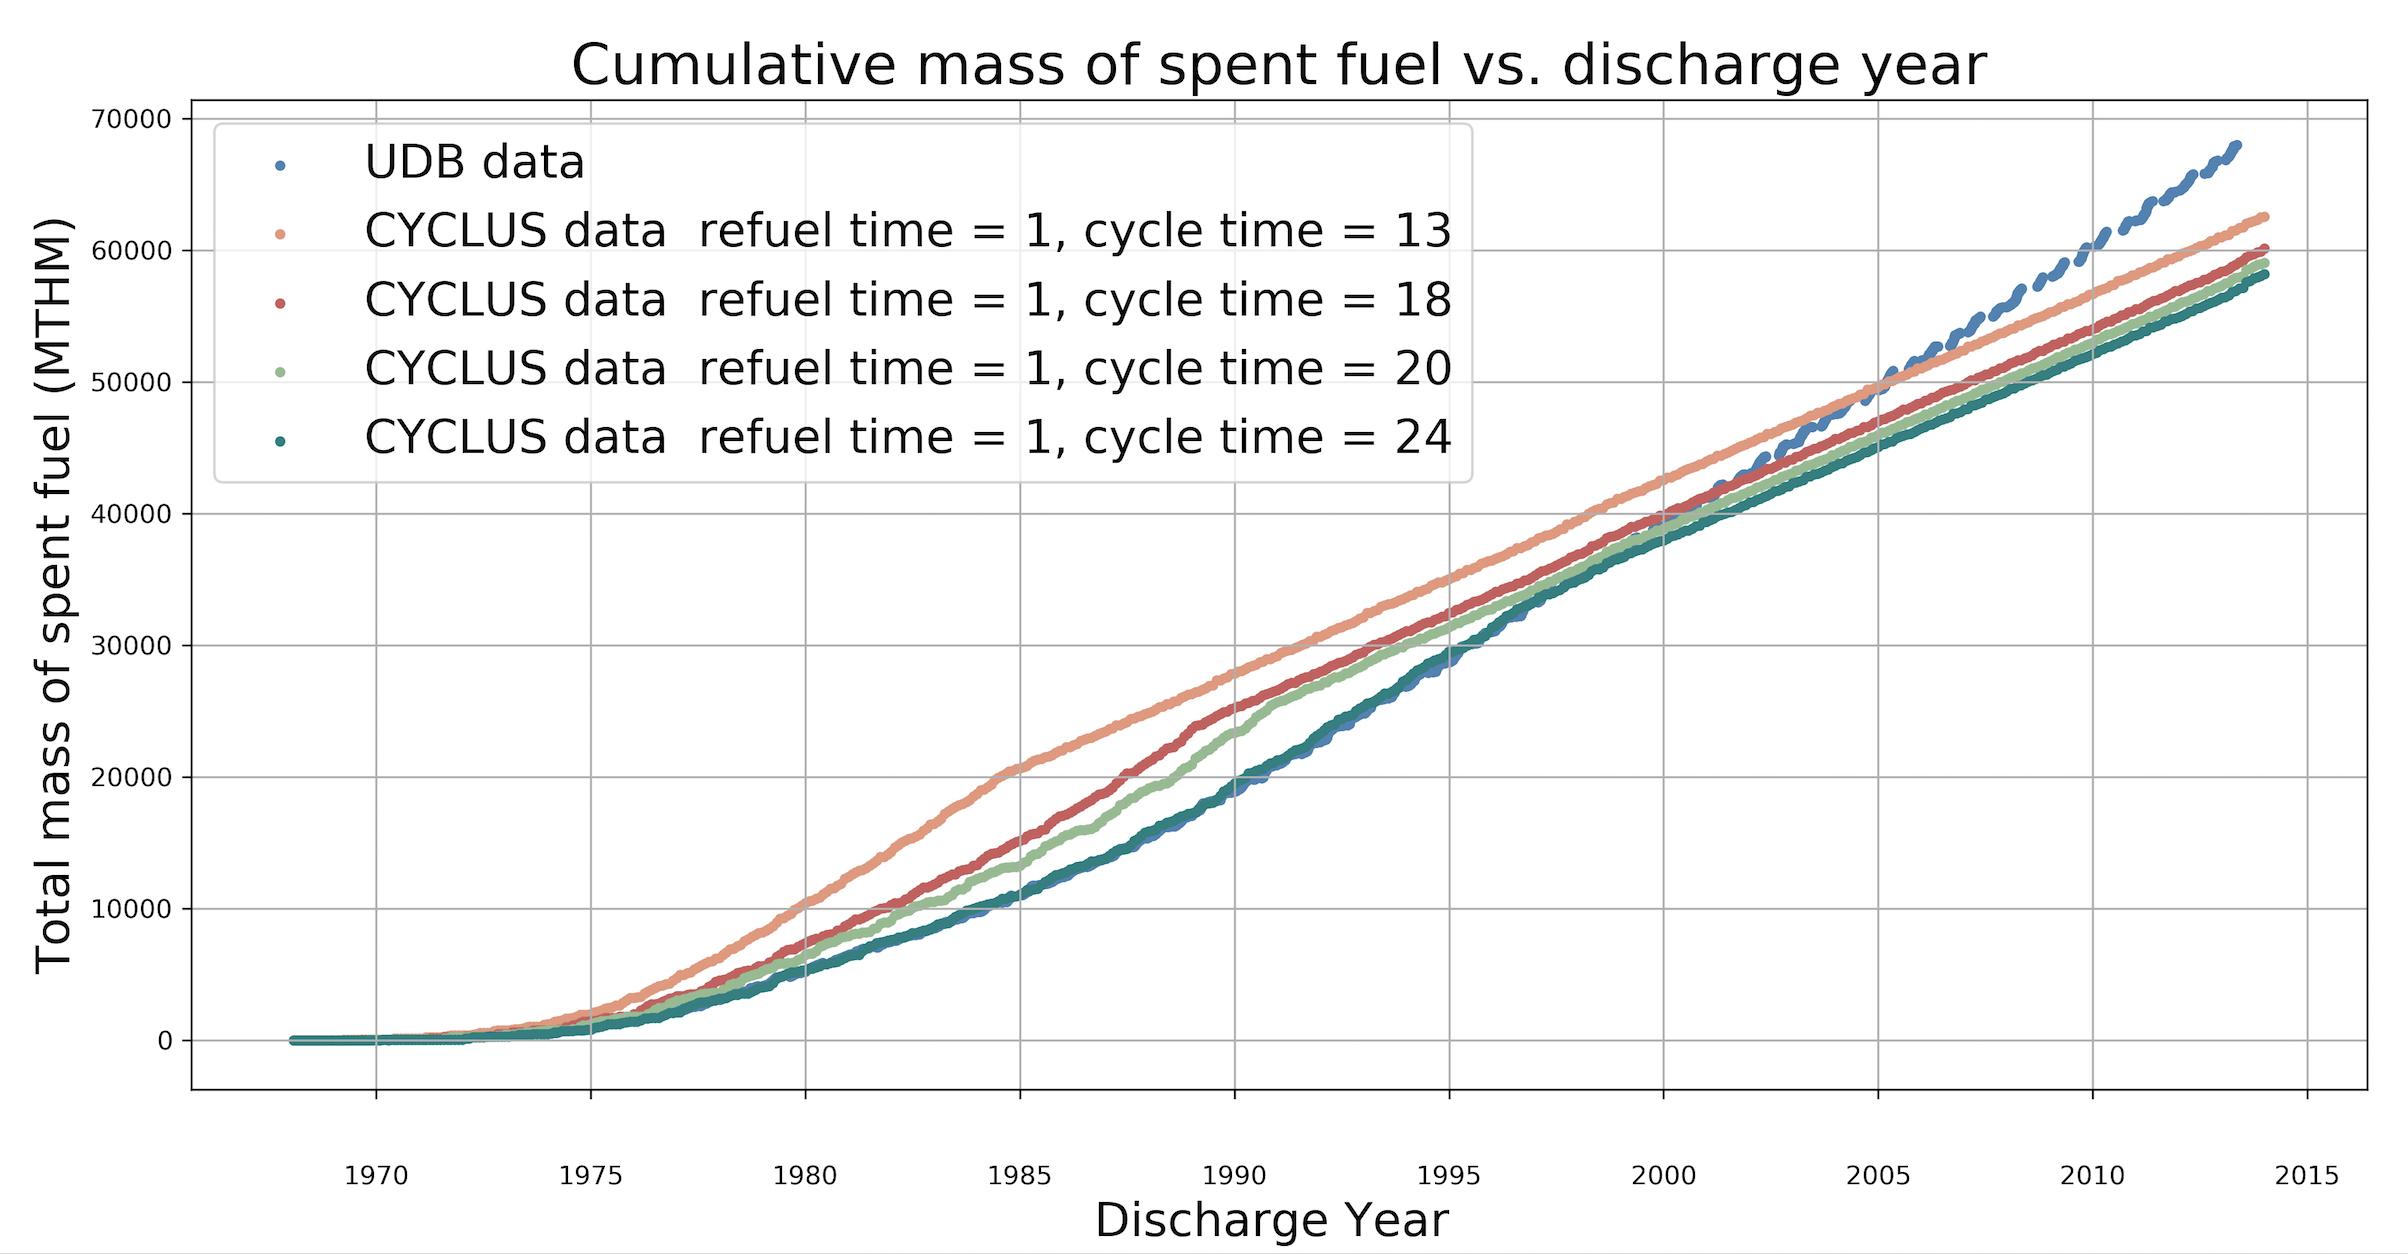
\includegraphics[width=0.48\textwidth]{figures/total_cumulative_mass_spent_fuel_cycletime}
	\caption{The total cumulative spent fuel mass against discharge time for \Cyclus and \gls{UDB} data from 1967 to 2013 for various cycle times.}
	\label{fig:total_cycletime}
\end{figure} 

The larger cumulative \gls{UDB} spent fuel mass compared to the \Cyclus simulation 
after 2000 can be attributed to the real world cycle lengths being shorter on 
average than the 18 month cycle time assumed in the  \Cyclus simulations. The 
\gls{US} \gls{DOE} reported that there was a downward trend of forced outage 
rates of nuclear reactors from 2000 to 2014. The forced outage rate was 4.24\% 
in 2000 and 2.98\% in 2013 \cite{gehin_nuclear_2016}. As the rate of forced 
outages decreased from 2000 to 2013, the cycle length also decreased. 

Figure \ref{fig:total_cycletime} plots total spent fuel mass from 
\Cyclus simulations where cycle duration is varied. A shorter cycle time brings the 
total spent fuel mass from \Cyclus simulations closer to the \gls{UDB} data after 
2000. 

\subsection{\textit{Major Isotopic Composition of  Spent Fuel Mass Comparison}}
To accurately simulate the U.S. nuclear fuel cycle from 1968 through the present, 
it important to use spent fuel recipes that have similar burnup in relation to 
the U.S. nuclear reactor burnup. 

Figure \ref{fig:burn_up_real} shows the average cumulative burnup for U.S. 
nuclear reactors from 1968 to 2013 \cite{eia_spent_2015}. Figure 
\ref{fig:burn_up_difference} shows the difference between burnup of the spent 
fuel recipes used in the \Cyclus simulations and cumulative burnup of U.S. 
nuclear reactors as seen in figure \ref{fig:burn_up_real}. On average, spent 
fuel burnup of 33 GWD/MTU is closer to the cumulative burnup of U.S. nuclear 
reactors than 51 GWD/MTU. 

\begin{figure}[t] % replace 't' with 'b' to force it to be on the bottom
	\centering
	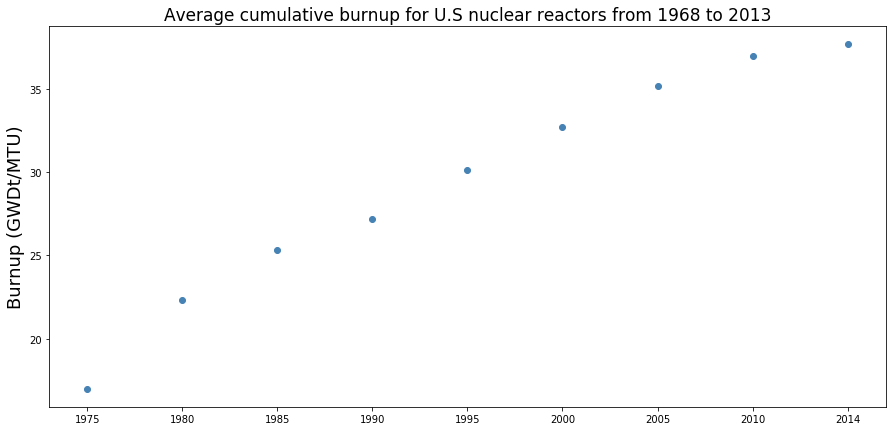
\includegraphics[width=0.48\textwidth]{figures/burn_up_real}
	\caption{The average cumulative burnup for U.S. nuclear reactors from 1968 to 2013 \cite{eia_spent_2015}.}
	\label{fig:burn_up_real}
\end{figure} 

\begin{figure}[t] % replace 't' with 'b' to force it to be on the bottom
	\centering
	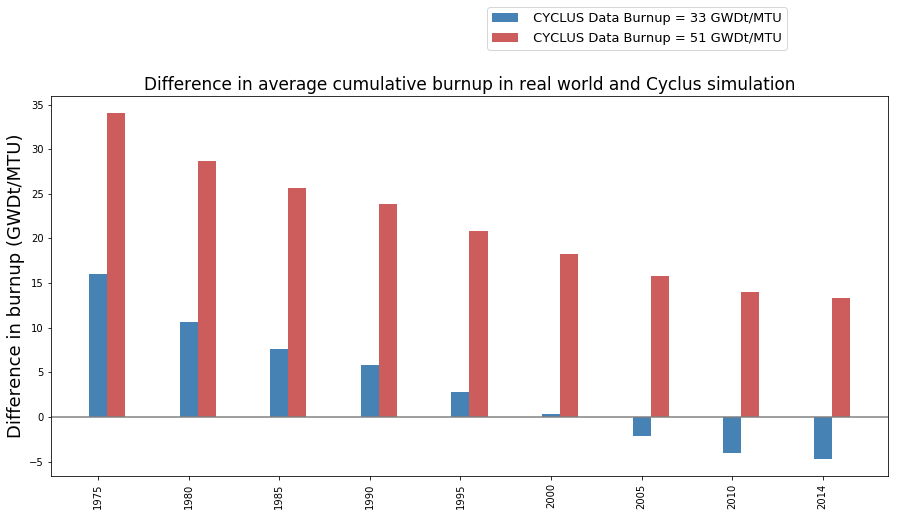
\includegraphics[width=0.48\textwidth]{figures/burn_up_difference}
	\caption{The difference between average cumulative burnup for U.S. nuclear reactors and burnup used in \Cyclus simulations.}
	\label{fig:burn_up_difference}
\end{figure} 

Figures \ref{fig:absolute_diff_all_51} and \ref{fig:absolute_diff_all_33} show 
the cumulative spent fuel isotopic mass difference between \gls{UDB} and \Cyclus data 
in 5 year intervals for burnup of 51 GWD/MTU and 33 GWD/MTU correspondingly. 
The \Cyclus data that had 33 GWD/MTU burnup deviated less compared to the 
\Cyclus data that had 51 GWD/MTU burnup. This is apparent for $^{236}$U, 
$^{242}$Pu and $^{240}$Pu. They are similar for the isotopes on the left side 
of both figures. With an exception of $^{239}$Pu having a substantial larger 
difference for 33 GWD/MTU than 51 GWD/MTU. 

\begin{figure*}[htb] % replace 't' with 'b' to force it to be on the bottom
	\centering
        \begin{subfigure}{0.9\textwidth}
        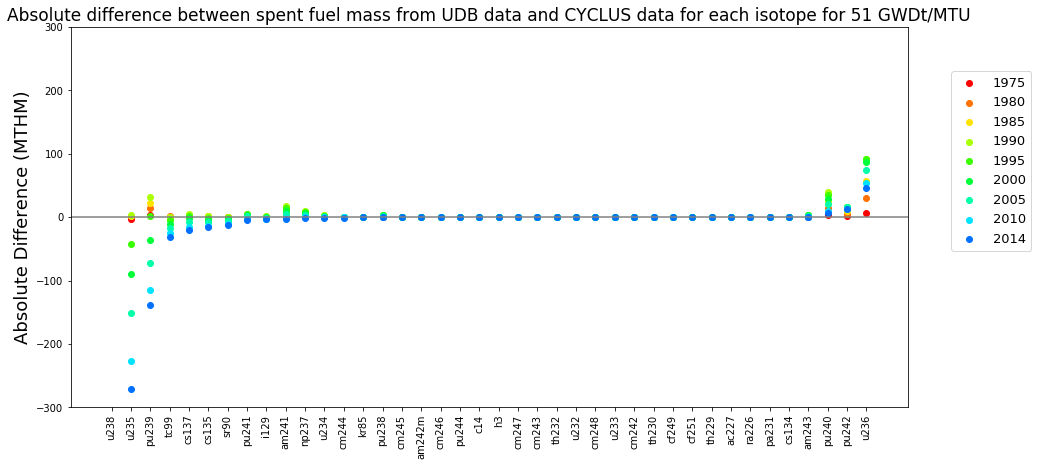
\includegraphics[height=0.30\textheight]{figures/absolute_diff_all_51}
        \caption{51 GWD/MTU burnup.}
	\label{fig:absolute_diff_all_51}
        \end{subfigure}
        \begin{subfigure}{0.9\textwidth}
        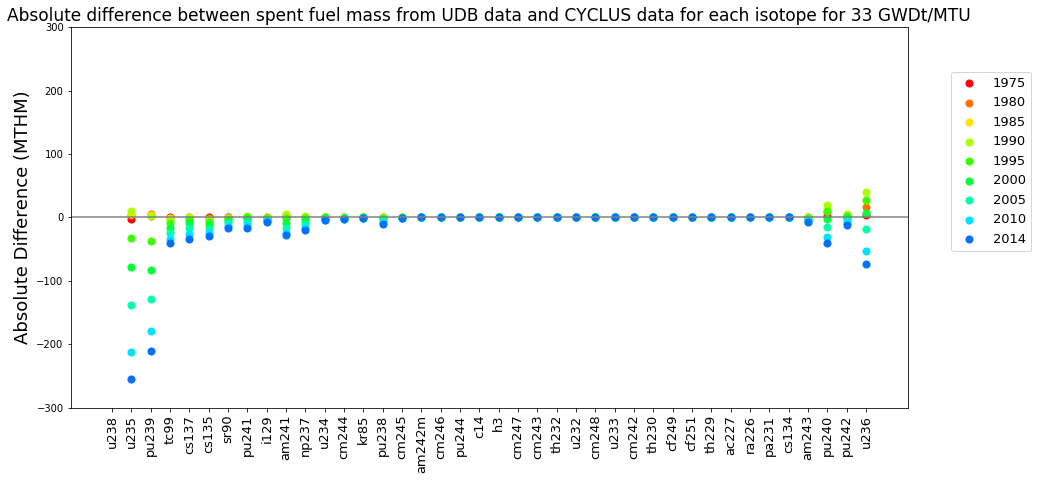
\includegraphics[height=0.30\textheight]{figures/absolute_diff_all_33}
        \caption{33 GWD/MTU burnup.}
	\label{fig:absolute_diff_all_33}
        \end{subfigure}
        \begin{subfigure}{0.9\textwidth}
        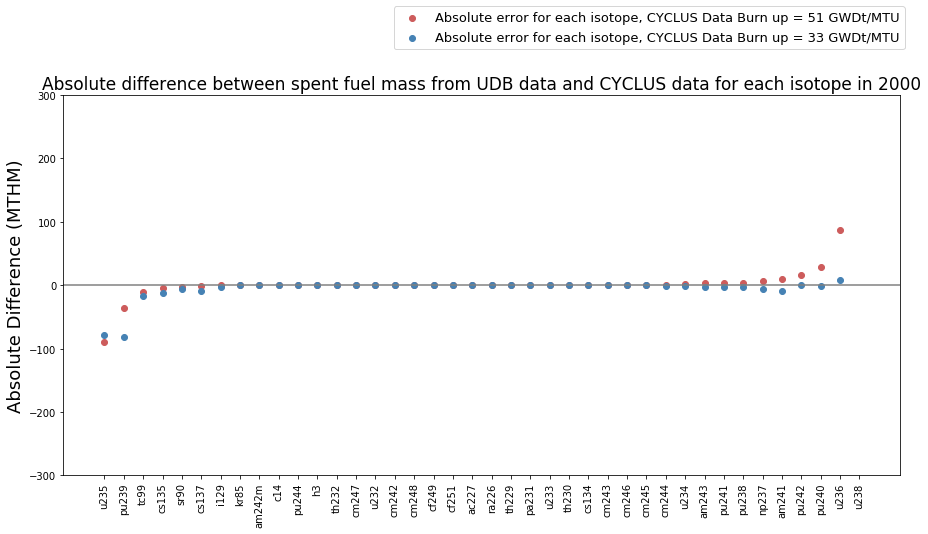
\includegraphics[height=0.35\textheight]{figures/absolute_diff_2000}
        \caption{Both burnup states, year 2000 data.}
	\label{fig:absolute_diff_2000}
        \end{subfigure}
        \caption{The absolute difference between spent fuel mass calculated by 
        \gls{UDB} and \Cyclus for each isotope. Positive difference indicates \Cyclus 
        mass estimate is larger.}
        \label{fig:absolute}
\end{figure*} 
\FloatBarrier

The 
cumulative spent fuel isotopic mass difference between \gls{UDB} and \Cyclus data for 
the year 2000 (figure \ref{fig:absolute_diff_2000}) demonstrates the impact of 
burnup on isotopic composition.  In figure 
\ref{fig:burn_up_real}, at year 2000, the cumulative average U.S. nuclear 
reactor burnup was very close to 33 GWD/MTU. Therefore, the difference in 
burnup between the U.S. nuclear reactor burnup and \Cyclus data burnup was 
around 20 GWD/MTU for 51 GWD/MTU burnup and 0 GWD/MTU for 33 GWD/MTU burnup 
(as seen in figure \ref{fig:burn_up_difference}). 

As discussed by Wigeland et al \cite{wigeland_separations_2006}, $^{240}$Pu, 
$^{239}$Pu and $^{241}$Am are the most significant long-term decay heat 
contributors to each waste package. While, $^{238}$Pu, $^{244}$Cm, $^{90}$Sr 
and $^{137}$Cs are the most significant short term decay heat contributors 
\cite{wigeland_separations_2006} to each waste package. 


In figure \ref{fig:absolute_diff_2000}, the \Cyclus simulation that uses the 33 
GWD/MTU burnup recipe has a small mass difference between \gls{UDB} and \Cyclus data 
for $^{240}$Pu and $^{241}$Am compared to 51 GWD/MTU burnup. However, it has a 
substantial difference for $^{239}$Pu. Figure 4 also shows small differences 
between \gls{UDB} and \Cyclus data for $^{238}$Pu, $^{244}$Cm, $^{90}$Sr and 
$^{137}$Cs. 

The large mass difference between \gls{UDB} and \Cyclus data (where \gls{UDB} $^{239}$Pu 
mass is larger than \Cyclus $^{239}$Pu mass) for $^{239}$Pu in figures 
\ref{fig:absolute_diff_2000}, \ref{fig:absolute_diff_all_51} and 
\ref{fig:absolute_diff_all_33} can be attributed to conservative depletion 
parameters used in the calculations for isotopic compositions in the \gls{UDB} 
database \cite{peterson_additional_2017}. These assumptions result in the 
hardening of the neutron spectrum that results in increased $^{239}$Pu 
production in the \gls{UDB} data \cite{peterson_additional_2017}. 

%%%%%%%%%%%%%%%%%%%%%%%%%%%%%%%%%%%%%%%%%%%%%%%%%%%%%%%%%%%%%%%%%%%%%%%%%%%%%%%%
\section{Conclusions}
This work demonstrates that the spent fuel mass and isotopic composition 
calculated by the \Cyclus simulation of the \gls{US} nuclear fuel cycle 
closely follow the results from real world metrics. This provides confidence 
that \Cyclus can be used to produce accurate isotopic decay heat contributions and 
simulate loading of a waste repository based on thermal constraints. 
To more closely replicate reality, future work will give the reactor agent the 
capability to accept varying cycle lengths, refueling durations and spent fuel 
recipes.

%%%%%%%%%%%%%%%%%%%%%%%%%%%%%%%%%%%%%%%%%%%%%%%%%%%%%%%%%%%%%%%%%%%%%%%%%%%%%%%%
\section{Acknowledgments}
This research is being performed using funding received from the \gls{DOE} Office of 
Nuclear Energy's Nuclear Energy University Program (Project 16-10512) 
"Demand-Driven Cycamore Archetypes". The authors want to thank members of the 
\gls{ARFC} group at the University of Illinois at Urbana-Champaign, 
particularly Jin Whan Bae and Gregory Westphal. We also thank our colleagues 
from the \Cyclus community, particularly those in the University of Wisconsin 
\gls{CNERG} and the University of South Carolina Energy Research Group (ERGS) 
for collaborative \Cyclus development.

%%%%%%%%%%%%%%%%%%%%%%%%%%%%%%%%%%%%%%%%%%%%%%%%%%%%%%%%%%%%%%%%%%%%%%%%%%%%%%%%
\bibliographystyle{ans}
\bibliography{bibliography}
\end{document}

